\documentclass{article}

\PassOptionsToPackage{numbers}{natbib}
\usepackage[preprint]{neurips_2025}

\usepackage[utf8]{inputenc}
\usepackage[T1]{fontenc}
\usepackage{hyperref}
\usepackage{url}
\usepackage{booktabs}
\usepackage{amsfonts}
\usepackage{amsmath}
\usepackage{amssymb}
\usepackage{nicefrac}
\usepackage{microtype}
\usepackage{xcolor}
\usepackage{graphicx}

\newcommand{\vw}{\mathbf{w}}
\newcommand{\vu}{\mathbf{u}}
\newcommand{\vc}{\mathbf{c}}
\newcommand{\vx}{\mathbf{x}}
\newcommand{\R}{\mathbb{R}}
\newcommand{\sign}{\operatorname{sign}}
\newcommand{\ins}{\mathcal{I}}

\title{CS771 Assignment 2: Bit-in-the-Middle Attack}

\author{%
  Group Member 1\thanks{Replace with actual group members and roll numbers.} \quad
  Group Member 2 \quad Group Member 3\\
  Department of Computer Science and Engineering\\
  Indian Institute of Technology Kanpur\\
}

\begin{document}

\maketitle

\begin{abstract}
We help Melbo learn a 17-bit arbiter PUF from challenge--response pairs (CRPs) whose middle
challenge bit was tampered with and then erased. We formulate the problem as latent-variable
maximum-likelihood estimation, apply the winner-take-all (hard-EM) approximation, and derive
alternating optimization algorithms for two latent priors: a non-informative uniform prior
(Part~1) and a structured prior in which the hidden bit is itself the response of a hidden
16-bit arbiter PUF (Part~3). We implement both algorithms using only \texttt{numpy} and
\texttt{sklearn} linear models, and analyse when and why their outputs agree or disagree
(Part~5).
\end{abstract}

\section{Notation and setup}

Each provided CRP is a pair $(\vc_i, r_i) \in \{0,1\}^{16} \times \{0,1\}$, $i \in [n]$,
$n = 8000$. For a challenge $\vc \in \{0,1\}^{16}$ and a bit $z \in \{0,1\}$, the insert
operation reconstructs a 17-bit challenge by placing $z$ in the middle (9-th) position:
$\ins(\vc, z) = [\vc[:8],\, z,\, \vc[8:]] \in \{0,1\}^{17}$.
Let $\phi_k : \{0,1\}^k \to \{-1,+1\}^k$ denote the standard arbiter-PUF embedding discussed
in class,
\begin{equation}
  \label{eq:phi}
  \big(\phi_k(\vc)\big)_j \;=\; \prod_{l = j}^{k} (1 - 2\,c_l), \qquad j \in [k],
\end{equation}
under which the response of a $k$-bit arbiter PUF is a linear (halfspace) function of
$\phi_k(\vc)$ \citep{ruhrmair2010modeling}. We write $\phi$ for both $\phi_{17}$ and
$\phi_{16}$, the arity being clear from context. Throughout, $\sigma(v) = 1/(1+e^{-v})$
denotes the sigmoid, $\tilde r_i \triangleq 2 r_i - 1 \in \{-1,+1\}$ and
$\tilde z_i \triangleq 2 z_i - 1 \in \{-1,+1\}$. We will repeatedly use the fact that
$-\ln \sigma(v) = \ln(1 + e^{-v}) \triangleq \ell(v)$ is the \emph{logistic loss}, a convex
and strictly decreasing function of $v$.

A useful structural observation follows directly from \eqref{eq:phi}: the inserted bit sits
at position $9$ of the 17-bit challenge, so flipping $z$ flips the sign of the factor
$(1 - 2z)$, and hence negates exactly the first $9$ coordinates of $\phi(\ins(\vc, z))$
while leaving coordinates $10,\dots,17$ unchanged:
\begin{equation}
  \label{eq:flip}
  \phi(\ins(\vc, 1)) = F\,\phi(\ins(\vc, 0)), \qquad
  F = \operatorname{diag}(\underbrace{-1,\dots,-1}_{9},\underbrace{+1,\dots,+1}_{8}).
\end{equation}
This lets us precompute both candidate embeddings for every CRP once, at the cost of one.

\section{Part 1: Alternating optimization with a uniform latent prior}

\paragraph{Deriving the objective.}
Melbo's likelihood model is
$P[r_i \mid z_i, \vc_i, \vw, b] = \sigma\!\big(\tilde r_i\,(\vw^\top \phi(\ins(\vc_i, z_i)) + b)\big)$
with the non-informative latent prior $P[z_i \mid \vc_i, \vw, b] = \nicefrac{1}{2}$.
Starting from the latent-variable MLE and applying the winner-take-all (WTA, also known as
\emph{hard-EM} or \emph{classification EM} \citep{celeux1992classification}) approximation,
i.e., replacing $\sum_{z_i}$ by $\max_{z_i}$, we obtain
\begin{align}
  \min_{\substack{(\vw, b)\\ \{z_i\}\in\{0,1\}^n}}
  \; -\sum_{i=1}^{n} \ln P[r_i, z_i \mid \vc_i, \vw, b]
  &= \min \; -\sum_{i=1}^{n} \Big( \ln P[r_i \mid z_i, \vc_i, \vw, b]
     + \ln \underbrace{P[z_i \mid \vc_i, \vw, b]}_{=\,1/2} \Big) \notag \\
  &= \min_{\substack{(\vw, b)\\ \{z_i\}}}
     \; \sum_{i=1}^{n} \ell\!\Big( \tilde r_i \big( \vw^\top \phi(\ins(\vc_i, z_i)) + b \big) \Big)
     \;+\; n \ln 2 .
  \label{eq:obj1}
\end{align}
The prior contributes only the constant $n \ln 2$, which can be dropped. Objective
\eqref{eq:obj1} is convex in $(\vw, b)$ for fixed $\{z_i\}$ but non-convex jointly (the
latents are discrete), which motivates \emph{alternating} (block-coordinate) optimization.

\paragraph{The $\{z_i\}$-step (latent update).}
For fixed $(\vw, b)$ the objective decomposes over $i$, so each $z_i$ can be updated
independently and \emph{exactly}. Since $\ell$ is strictly decreasing,
\begin{equation}
  \label{eq:zstep1}
  z_i \;\leftarrow\; \underset{z \in \{0,1\}}{\arg\min}\;
  \ell\!\Big( \tilde r_i \big( \vw^\top \phi(\ins(\vc_i, z)) + b \big) \Big)
  \;=\; \underset{z \in \{0,1\}}{\arg\max}\;
  \tilde r_i \big( \vw^\top \phi(\ins(\vc_i, z)) + b \big),
\end{equation}
i.e., each CRP greedily picks the middle bit whose (signed) score best explains its observed
response --- a per-point winner-take-all step. Using \eqref{eq:flip}, both candidate scores
$s_i^{(0)} = \vw^\top \phi(\ins(\vc_i, 0)) + b$ and $s_i^{(1)} = \vw^\top F\,\phi(\ins(\vc_i, 0)) + b$
are computed with vectorized matrix products; the whole step is $O(n \cdot 17)$.

\paragraph{The $(\vw, b)$-step (model update).}
For fixed $\{z_i\}$, define completed feature vectors $\vx_i \triangleq \phi(\ins(\vc_i, z_i))$.
The subproblem
\begin{equation}
  \label{eq:wstep1}
  (\vw, b) \;\leftarrow\; \underset{(\vw, b) \in \R^{17}\times\R}{\arg\min}\;
  \sum_{i=1}^{n} \ell\!\big( \tilde r_i (\vw^\top \vx_i + b) \big)
  \;\Big(+\, \tfrac{1}{2C}\|\vw\|_2^2\Big)
\end{equation}
is exactly \emph{logistic regression} of the labels $r_i$ on the features $\vx_i$: a convex
problem solved to (near) global optimality by any standard solver. We use
\texttt{sklearn.linear\_model.LogisticRegression}; the small $\ell_2$ term (inverse strength
$C$) is added for numerical stability, since the completed data is often linearly separable
and the unregularized MLE would diverge in norm.

\paragraph{The algorithm and its convergence.}
Initialize $z_i \overset{iid}{\sim} \text{Bernoulli}(\nicefrac12)$ and repeat
\eqref{eq:wstep1} then \eqref{eq:zstep1} until $\{z_i\}$ stops changing (or an iteration cap
is hit). Every step solves its block subproblem exactly, hence the objective
\eqref{eq:obj1} is monotonically non-increasing; being bounded below and with finitely many
latent configurations, the procedure terminates at a partial optimum in finitely many
alternations. The problem is non-convex and sensitive to initialization, so we run several
random restarts and keep the $(\vw, b, \{z_i\})$ triple with the best training-response
accuracy. This is precisely what \texttt{my\_latent()} implements.

\section{Part 3: Alternating optimization with a PUF-structured latent prior}

Melba's intelligence changes the latent prior: the middle bits are responses of a hidden
16-bit arbiter PUF $(\vu, a) \in \R^{16}\times\R$,
\begin{equation*}
  P[r_i \mid z_i, \vc_i, \vw, b, \vu, a]
    = \sigma\!\big(\tilde r_i (\vw^\top \phi(\ins(\vc_i, z_i)) + b)\big),
  \qquad
  P[z_i \mid \vc_i, \vw, b, \vu, a]
    = \sigma\!\big(\tilde z_i (\vu^\top \phi(\vc_i) + a)\big).
\end{equation*}

\paragraph{Deriving the objective.}
The MLE problem $\max \prod_{i=1}^n P[r_i \mid \vc_i, \vw, b, \vu, a]$ marginalizes over the
latent bits,
\begin{equation*}
  P[r_i \mid \vc_i, \vw, b, \vu, a]
  = \sum_{z_i \in \{0,1\}} P[r_i \mid z_i, \vc_i, \vw, b]\; P[z_i \mid \vc_i, \vu, a].
\end{equation*}
Introducing the latents explicitly, applying WTA ($\sum_{z_i} \to \max_{z_i}$), and taking
negative logs yields the joint minimization
\begin{equation}
  \label{eq:obj2}
  \min_{\substack{(\vw, b),\, (\vu, a)\\ \{z_i\} \in \{0,1\}^n}}
  \; \sum_{i=1}^{n} \Big[
     \underbrace{\ell\!\big( \tilde r_i (\vw^\top \phi(\ins(\vc_i, z_i)) + b) \big)}_{\text{response likelihood}}
     \;+\;
     \underbrace{\ell\!\big( \tilde z_i (\vu^\top \phi(\vc_i) + a) \big)}_{\text{latent prior likelihood}}
  \Big].
\end{equation}
There are now three natural blocks, each of which we can optimize exactly.

\paragraph{The $\{z_i\}$-step.}
For fixed models, \eqref{eq:obj2} again decomposes over $i$, but each latent bit is now
scored by the \emph{joint} likelihood of both PUFs. Writing
$s_i^{(z)} = \vw^\top \phi(\ins(\vc_i, z)) + b$ and $t_i = \vu^\top \phi(\vc_i) + a$,
\begin{equation}
  \label{eq:zstep2}
  z_i \;\leftarrow\; \underset{z \in \{0,1\}}{\arg\max}\;
  \Big[ \ln \sigma\!\big( \tilde r_i\, s_i^{(z)} \big)
      + \ln \sigma\!\big( (2z - 1)\, t_i \big) \Big] .
\end{equation}
The second term acts as a data-dependent prior: a CRP may no longer pick whichever bit best
explains its response if that bit is implausible under the hidden 16-bit PUF.

\paragraph{The $(\vw, b)$-step.}
For fixed $\{z_i\}$ and $(\vu, a)$, the second summand of \eqref{eq:obj2} is constant, and we
recover exactly subproblem \eqref{eq:wstep1}: logistic regression of the responses $r_i$ on
the completed 17-bit embeddings $\phi(\ins(\vc_i, z_i))$.

\paragraph{The $(\vu, a)$-step.}
Symmetrically, for fixed $\{z_i\}$ and $(\vw, b)$, the first summand is constant and
\begin{equation}
  \label{eq:ustep}
  (\vu, a) \;\leftarrow\; \underset{(\vu, a) \in \R^{16}\times\R}{\arg\min}\;
  \sum_{i=1}^{n} \ell\!\big( \tilde z_i (\vu^\top \phi(\vc_i) + a) \big)
  \;\Big(+\, \tfrac{1}{2C}\|\vu\|_2^2\Big),
\end{equation}
which is logistic regression of the \emph{current latent estimates} $z_i$ (treated as labels)
on the 16-bit embeddings $\phi(\vc_i)$. In other words, the hidden PUF is learnt by mounting
a standard linear model-extraction attack on our own current guesses of the middle bits.

\paragraph{The algorithm.}
Initialize $z_i \overset{iid}{\sim} \text{Bernoulli}(\nicefrac12)$ and cycle
\eqref{eq:wstep1} $\to$ \eqref{eq:ustep} $\to$ \eqref{eq:zstep2} until the latents stabilize.
Each block update is exact, so objective \eqref{eq:obj2} decreases monotonically and the same
convergence argument as in Part~1 applies. One practical safeguard: if the latent vector ever
collapses to a single class (all $z_i$ equal), step \eqref{eq:ustep} is ill-posed, so we
re-randomize a small fraction of the latents. As before we use random restarts; restarts are
compared by the accuracy of the \emph{deployment pipeline} that the evaluator will actually
use --- predict $\hat z_i = \mathbf{1}[\vu^\top \phi(\vc_i) + a > 0]$, then predict the
response with $(\vw, b)$ on $\phi(\ins(\vc_i, \hat z_i))$. This is what
\texttt{my\_latent\_updated()} implements; it returns only $(\vw, b, \vu, a)$ since the
latents for unseen CRPs are now \emph{predicted} by the 16-bit model rather than being free
parameters.

\section{Part 5: Do the two algorithms agree?}

Table~\ref{tab:results} and Figure~\ref{fig:conv} summarize our runs on the released
public dataset (8000 train / 2000 test CRPs).\footnote{To probe recovery of the (unknown)
true middle bits, we additionally \emph{replicated} the data-generation process described in
the assignment with PUFs of our own (so that ground truth is known) and repeated all
experiments; those replication numbers are called out explicitly where used.}
Writing $(\vw, b, \{z_i\})$ for the output of \texttt{my\_latent()} and
$(\tilde\vw, \tilde b, \tilde\vu, \tilde a)$ for the output of
\texttt{my\_latent\_updated()}, we observed:
\begin{enumerate}
  \item[(a)] \textbf{No, $\vw \not\approx \tilde\vw$.} The cosine similarity between the two
  (normalized) weight vectors was $\approx +0.46$ on the public data ($\approx -0.41$ after
  accounting for the flip symmetry described below) --- moderately correlated at best, far
  from equal. Norms differ as well, which is expected: on (near-)separable completed data the
  logistic MLE direction is what matters while the scale is set by the regularizer, so at
  best the directions could agree.
  \item[(b)] \textbf{No, $b \not\approx \tilde b$} ($b \approx -0.57$ vs
  $\tilde b \approx -1.64$ in our run).
  \item[(c)] The fraction of train CRPs with
  $2 z_i - 1 = \sign(\tilde\vu^\top \phi(\vc_i) + \tilde a)$ was $\approx 0.64$. Moreover,
  this number is not stable: re-running \texttt{my\_latent()} from 10 different random
  initializations gave fractions scattered over $[0.34, 0.66]$ --- roughly symmetric around
  chance level $\nicefrac12$ --- even though every one of those runs fit the training
  responses at $\geq 99.7\%$ accuracy. In our ground-truth replication experiment, the
  $\{z_i\}$ of \texttt{my\_latent()} agreed with the true middle bits on only $\approx 56\%$
  of CRPs (chance, up to a global flip), whereas the bits predicted by
  $(\tilde\vu, \tilde a)$ agreed with the ground truth on $\approx 99.6\%$.
\end{enumerate}

\begin{table}[t]
  \caption{Results on the released public dataset (single machine, \texttt{sklearn} LBFGS
  solver). Test accuracy for \texttt{my\_latent\_updated()} uses the official pipeline:
  middle bits predicted by $(\tilde\vu, \tilde a)$, responses by $(\tilde\vw, \tilde b)$.}
  \label{tab:results}
  \centering
  \begin{tabular}{lccc}
    \toprule
    Method & Wall time & Train accuracy & Test accuracy \\
    \midrule
    \texttt{my\_latent()} (own latents) & $0.11$ s & $0.9998$ & --- \\
    \texttt{my\_latent\_updated()} (predicted latents) & $2.8$ s & $0.9964$ & $0.9970$ \\
    \bottomrule
  \end{tabular}
\end{table}

\begin{figure}[t]
  \centering
  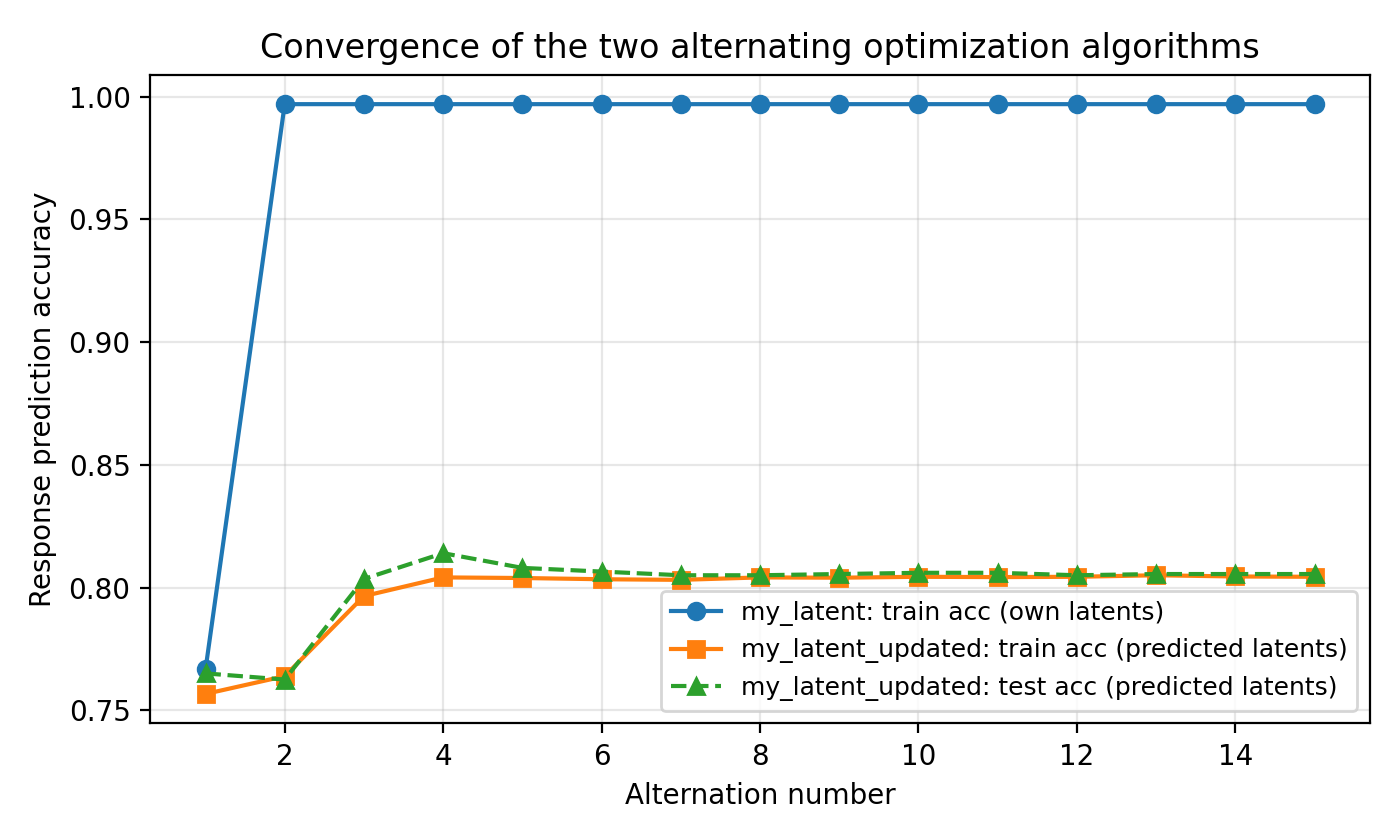
\includegraphics[width=0.78\linewidth]{convergence.png}
  \caption{Response-prediction accuracy versus alternation number for the two algorithms
  (single restart each). \texttt{my\_latent} evaluates with its own latent bits;
  \texttt{my\_latent\_updated} evaluates with the deployment pipeline
  ($\hat z$ from the 16-bit model, then the 17-bit model).}
  \label{fig:conv}
\end{figure}

\paragraph{Why the disagreement is expected.}
Three effects are at play.

\emph{(i) An exact flip symmetry makes the models identifiable only up to a global flip.}
By \eqref{eq:flip}, the transformation $z_i \mapsto 1 - z_i$ for all $i$ together with
$\vw \mapsto F\vw$ leaves every likelihood term in \eqref{eq:obj1} unchanged; in Part~3 the
same holds after additionally mapping $(\vu, a) \mapsto (-\vu, -a)$. So even two perfect
runs could only agree up to this symmetry (the fraction in (c) would then be $\approx 1$ or
$\approx 0$). This is why we report all comparisons ``up to a global flip''. Our observed
fractions ($0.64$ in the main run, scattered over $[0.34, 0.66]$ across initializations) sit
around $\nicefrac12$ and never approach $0$ or $1$, i.e., the disagreement is real, not a
flip artifact.

\emph{(ii) Part~1's problem is massively under-determined.} With a uniform prior, the $8000$
latent bits are completely free: the effective hypothesis class is
$\{(\vw, b)\} \times \{0,1\}^{8000}$, and the objective only asks that \emph{some} completion
of each challenge be consistent with its response. Per-CRP freedom is enough to drive the
training loss to (near) zero from almost any initialization --- all $10$ of our random
initializations reach $\geq 99.7\%$ (often $100\%$) training accuracy within a handful of
alternations, yet produce mutually inconsistent latent assignments --- so there is a huge set
of near-global optima, and hard-EM simply lands on whichever one its initialization is
attracted to. Nothing in the objective rewards recovering the \emph{true} middle bits, and in
our ground-truth replication the recovered $\{z_i\}$ were at chance level with respect to
them. This is classic overfitting through latent variables: WTA lets each point ``explain
away'' its response.

\emph{(iii) Part~3's structured prior collapses the latent capacity and identifies the truth.}
Constraining the middle bits to be realizable as $\sign(\vu^\top \phi(\vc_i) + a)$ replaces
the $2^{8000}$ free latent configurations by only those labelings achievable by a
17-parameter halfspace over $\phi(\vc)$ --- by Sauer's lemma, at most
$O(n^{17})$ of them \citep{shalev2014understanding}, an astronomically smaller and, crucially,
\emph{correctly specified} class (the data really was generated this way). Fitting the train
responses now forces the algorithm towards the true latent structure: in our ground-truth
replication the learnt $(\tilde\vu, \tilde a)$ reproduced the true middle bits on
$\approx 99.6\%$ of CRPs (up to flip), and on the public dataset the pipeline generalizes to
unseen test CRPs at $99.7\%$ --- which the Part~1 model, whose latents are undefined for new
points, cannot even attempt.

In short: the two algorithms disagree because they solve genuinely different problems. The
first fits the training responses (perfectly) without identifying the data-generating process;
the second, thanks to the informative prior, identifies (nearly) the true pair of PUFs, and
consequently its $(\tilde\vw, \tilde b, \tilde\vu, \tilde a)$ bears no particular resemblance
to the arbitrary near-optimum found by the first.

\begin{thebibliography}{9}

\bibitem{ruhrmair2010modeling}
U.~R\"uhrmair, F.~Sehnke, J.~S\"olter, G.~Dror, S.~Devadas, and J.~Schmidhuber.
\newblock Modeling attacks on physical unclonable functions.
\newblock In \emph{Proceedings of the 17th ACM Conference on Computer and Communications
Security (CCS)}, 2010.

\bibitem{celeux1992classification}
G.~Celeux and G.~Govaert.
\newblock A classification {EM} algorithm for clustering and two stochastic versions.
\newblock \emph{Computational Statistics \& Data Analysis}, 14(3):315--332, 1992.

\bibitem{dempster1977maximum}
A.~P. Dempster, N.~M. Laird, and D.~B. Rubin.
\newblock Maximum likelihood from incomplete data via the {EM} algorithm.
\newblock \emph{Journal of the Royal Statistical Society: Series B}, 39(1):1--38, 1977.

\bibitem{shalev2014understanding}
S.~Shalev-Shwartz and S.~Ben-David.
\newblock \emph{Understanding Machine Learning: From Theory to Algorithms}.
\newblock Cambridge University Press, 2014.

\end{thebibliography}

\end{document}
